\documentclass[]{article}
\usepackage{amssymb}
\usepackage{amstext}
\usepackage{graphicx} 

\newtheorem{theorem}{Theorem}
\newtheorem{proof}{Proof}
\newtheorem{definition}{Definition}
\newtheorem{claim}{Claim}

%opening
\title{Neural Networks Can Approximate Continuous Functions}
\author{Paul Dubois}
\date{}

\begin{document}

\maketitle

\begin{abstract}
	A clean Tex version of the proof seen during the lectures that neural networks with ReLU activation can approximate continuous functions.
\end{abstract}

\begin{definition}
	$\mathcal{C}\left( \left[ a,b \right] \right)$ is the set of real continuous functions on $\left[ a,b \right]$.
\end{definition}
\begin{definition}
	$\mathcal{P}\left( n,l \right)$ is the set of rectangle 1D-1D perceptrons with $l$ hidden layers and $n$ neurons in each hidden layer.
\end{definition}

\section{Theorem}
$$\forall f \in \mathcal{C}(\left[ a,b \right]), \ \forall \varepsilon > 0, \ \exists N \in \mathbb{N} \text{ and } p \in \mathcal{P}(N,1) \text{ s.t. } \|p-f\|_\infty < \varepsilon$$
Where $\|g\|_\infty$ is infinity norm of $g$ on $\left[ a,b \right]$; i.e. $\|g\|_\infty = \max_{x \in \left[ a,b \right]}(|g(x)|)$.

\section{Idea}

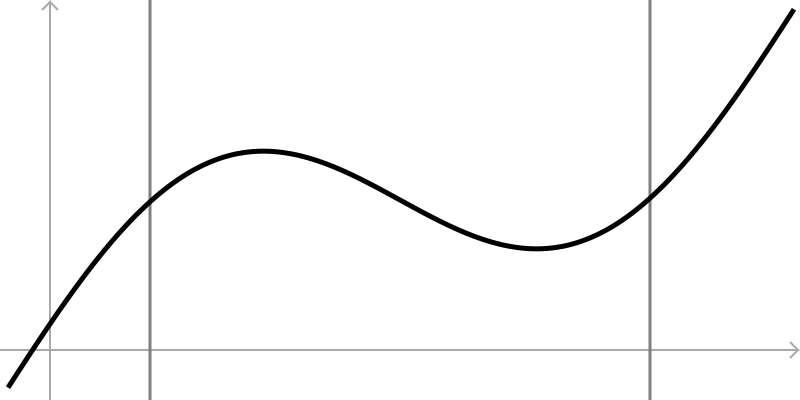
\includegraphics[width=\linewidth]{plot}

\section{Proof}


\end{document}
